\chapter{Background \& Objectives}

%This section should discuss your preparation for the project, including background reading, your analysis of the problem and the process or method you have followed to help structure your work.  It is likely that you will reuse part of your outline project specification, but at this point in the project you should have more to talk about. 



%\begin{itemize}
%   \item All of the sections and text in this example are for illustration purposes. The main Chapters are a good starting point, but the content and actual sections that you include are likely to be different.
   
 %  \item Look at the document on the Structure of the Final Report for additional guidance. 
   
%\end {itemize}

\section{Background}
\subsection{Introduction}

This project uses data and images collected during the course of experiments conducted at the National Plant Phenomics Centre (NPPC)\cite{_nppc}. The NPPC, based near Aberystwyth, houses a state-of-the-art, automated greenhouse and imaging system. During experiments, plants are housed on moving conveyors and are carried one by one through measurement chambers where images of various modalities (such as infra red and visible light) are captured from multiple angles. Physical and environmental measurements, such as plant weight, water usage or greenhouse temperatures, can also be captured automatically. More specific or specialist data (such as targeted phenotype or genotype traits) are captured following observation by staff at the facility.

The experiments at the NPPC are capable of investigating large sets of plants including whole breeding populations in order to inform how physical characteristics are affected by genes. Phenotyping experiments will often conduct a quantitative trait locus (QTL) analysis where sections of DNA corresponding to certain desirable phenotypes are identified, mapped and recorded for consideration in future breeding. The NPPC is capable of supporting a wide range of plants, from food-security critical cereal crops such as wheat and oats to plants that are promising sources of bio-fuel or biomass such as Miscanthus. The results of these experiments can directly affect the yield and robustness of future generations of important crops.

There is a wealth of data collected at the NPPC that is often never considered again following the conclusion of an experiment. This project seeks to provide an ongoing use for some of these data and images.

\subsection{Initial project topic}
The initial title for this project was `Building a plant Atlas from real images'.  In this context an Atlas is a term used to describe a visual reference for developmental stages within a subject of interest. Such an approach is commonly attributed to Tanner et al \cite{tanner_assessment_1975} for their work at numerically scoring the stages of bone development within the hands of infants and providing a visual reference for each stage. 

Biologists use numerical growth stage indices to chart the developmental milestones in the life cycle of a given plant. In cereals a popular scale for these growth stages is the 0 to 100 scale defined by Zadoks \cite{zadoks_decimal_1974} in 1974. These scales are often presented in an Atlas style with hand drawn, stylised images used to display detail of the characteristics of a particular growth stage. Figure~\ref{fig:bbch} shows an example taken from the BBCH scale which is based on the Zadoks cereal scale.

\begin{figure}[H]
    \centering
    
\includegraphics[width=\textwidth]{images/background/bbchscale}
    \caption{Example of `atlas' style visualisation of wheat plant development stages. Source : Wikimedia Commons \cite{bbch_scale}}
    \label{fig:bbch}
\end{figure}



 The aim of the original project was to utilise the images and data collected during a particular experiment at the NPPC in order to provide an atlas style visualisation using real plant images and providing a web based interface onto this visualisation with the intention of it being used as a reference for the biologists or a teaching aid and to sort or align the experiment population on growth stage and compare their physical characteristics. Further suggested work on this topic was to leverage some machine learning capability to attempt to draw conclusions or infer useful correlations from the datasets collected over the course of running experiments.

This topic was selected for the subject of this dissertation since it provided a chance at building a system that may have some practical use and application after the dissertation was complete. The topic also provided the opportunity to learn about certain plants, their life cycles and their importance as a research subject, this seemed like a more interesting problem domain when compared to other available choices.

\subsection{Change of project topic}\label{changeproj}

In the initial weeks of the project, meetings were arranged with Dr Roger Boyle, a researcher specialising in computer vision based applications at the NPPC. The purpose of these meetings was to discuss the direction and background of the originally proposed project and arrange visits to the NPPC itself in order to gain an understanding of the facility and its functions. Spike work, prototyping and research into plants, growth stages, atlases and investigations into agreement between expert opinions \cite{williams_comparing_1976} were the focus of these early weeks as opposed to investigations into the data being collected at the NPPC.

 In order for the original topic to be successful, the recording of key growth stage information during the course of an experiment was necessary, without these data points it would not be possible to build the proposed atlas visualisations. Unfortunately, where it was assumed that such data was being recorded as a matter of course during NPPC experiments, it became apparent that the recording of plant characteristics data during experiments was extremely sparse. When experiment data was provided for analysis it became clear that the approach to data collection was very different from what was expected. 
 
 The interdisciplinary differences in attitude to data between the computer scientists and biologists involved was a key factor in the erroneous assumptions regarding the quantity and quality of collected data. The biologists who collect experiment data are often concerned only with growth stages which are directly associated with traits that are being targeted as part of the experiment and from the data analysed are content with error margins of up to three days. 
 
 With only a handful of growth stages captured it became clear that the original project topic would not be possible. Following this discovery a meeting was arranged with various staff at the NPPC including the director, Professor John Doonan, in order to discuss what data was available and what would be a useful project. The outcome of this meeting was a new project topic, a system would be implemented that would make use of available images and data for a given experiment and present it in an easy to navigate fashion. The produced system should also natively support the means to add additional data to an experiment such that a more complete dataset could potentially be achieved and saved in a web-accessible database. 
 
 %The produced system would provide the means to explore collected data whilst linking these data back to the various images of the associated plants.
 
 %The system would link with the NPPC data repository and use it as the source of available experiments and the image data associated with them. Experiment data would need to be imported or added manually via some provided facility within the produced system.
 
 
  

\subsection{Existing solutions}
Two alternative solutions were investigated during the discovery stages of this project. The first is the current means for experiment images to be viewed at the NPPC. Figure~\ref{fig:acc_phe} shows an excerpt from an internal webpage hosted by the NPPC that provides access to the plant images associated with a particular experiment. Here we can see the available image modalities and can select between the various image angles. Following one of these links will display the entire time series(days) of captured images for the plant corresponding to the chosen modality and angle. Whilst this system allows browsing of the images captured it does not allow a simple way to compare or switch between the different modalities of images that correspond to the same time (day) in the life of the plant. No means to view or add associated plant data is available in this solution.

\begin{figure}[H]
    \centering
    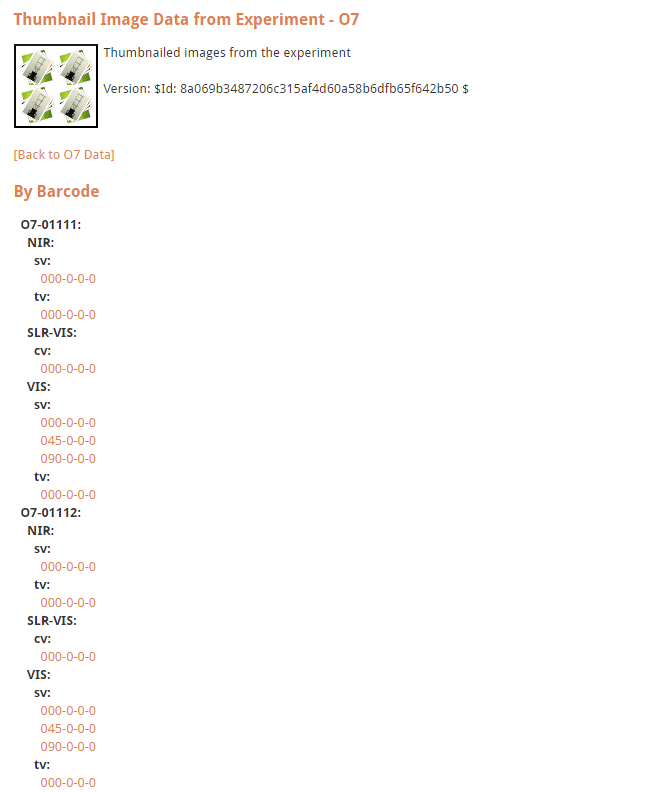
\includegraphics[width=0.7\textwidth]{images/background/access_phen}
    \caption{Current means of NPPC image exploration}
    \label{fig:acc_phe}
\end{figure}

The second existing solution investigated is a commercial product called Zegami\cite{_Zegami} developed in part by Oxford University. Figure~\ref{fig:zegami} shows the Zegami system in action on the Australian Plant Phenomics Facility\cite{_aus} website. Zegami is a web based tool that allows the browsing of large amounts of images in a fairly intuitive and responsive way and also provides the means to search, sort and filter images using associated data attributes. Zegami allows the visualisation of data in graphical formats and provides the means to select subsections of the images based on selections made in the graphical views via drawing boxes or circles around the desired datapoints.

Being positioned as a image and data exploration tool, data addition is mostly done from a single datasource file in Zegami with no out-of-the-box facility for users to add supplementary data to an experiment.

Zegami is a feature-rich and robust solution for exploring large collections of images and associated data, however, being a commercial venture it is not free and can be considered prohibitively expensive a solution for a project of this nature.


\begin{figure}[H]
    \centering
    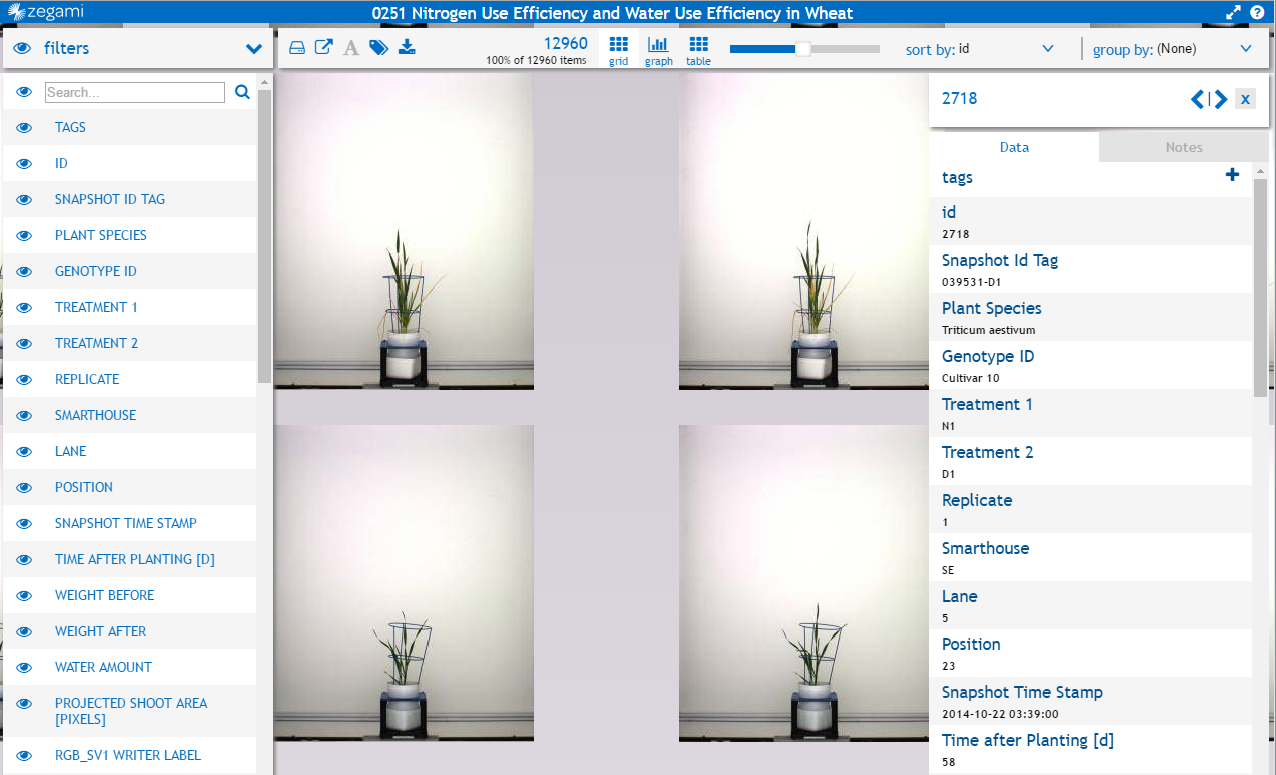
\includegraphics[width=0.7\textwidth]{images/background/zegami}
    \caption{Zegami system as used by the Australian Plant Phenomics Facility. Source : \url{https://zegami.plantphenomics.org.au}}
    \label{fig:zegami}
\end{figure}
\section{Analysis}
%Taking into account the problem and what you learned from the background work, what was your analysis of the problem? How did your analysis help to decompose the problem into the main tasks that you would undertake? Were there alternative approaches? Why did you choose one approach compared to the alternatives? 

%There should be a clear statement of the objectives of the work, which you will evaluate at the end of the work. 

The core problem that this project aims to solve is the need for a web-based system that enables the exploration of images and associated data that are collected during experiments at the NPPC. 


 Following the domain research and familiarisation with the NPPC gained during the discovery period for the initial project specification it was felt that the new direction of the project was well understood and that certain requirements could be identified fairly quickly. The following list will detail these and further additional requirements identified during the course of the project to provide a complete view of targeted functional specifications.


\subsection{Requirements decomposition}

%In most cases, the agreed objectives or requirements will be the result of a compromise between what would ideally have been produced and what was felt to be possible in the time available. A discussion of the process of arriving at the final list is usually appropriate.

\subsubsection{Web based system} In order to provide a practical solution to the problem, access to the system should be available from a wide array of devices and systems. The system should also be accessible from a variety of different locations. The most practical solution to these considerations is a web based approach. Most devices and systems natively support some kind of web access and a centrally hosted solution is far more accessible than any alternative approach.


\subsubsection{Integrate with NPPC data repository} The system needs to display plants, plant images and associated data. Data and images captured at the NPPC during experiments are stored in a central data repository hosted on the Aberystwyth University network. In order to provide access to these images and data via a web based approach, it is necessary to integrate the system with the data repository such that the images or data can be pulled directly from the repository as opposed to re-hosting the same content within the delivered system itself. The sheer quantity of image data in the repository itself makes a re-hosting solution highly impractical. 

 
\subsubsection{Browse plants and plant images}  Users will be able to view plants, associated data and plant images. In order to provide a means of exploring the data and images captured at the NPPC, the system needs to provide some interface onto these data that allows easy navigation between plants, images and associated data. Currently there is no consolidated interface onto both experiment images and the data observations captured during the course of experiments. Providing such an interface makes the exploration of past and current experiments convenient and simple.

\subsubsection{Import experiment data}  Experiment data will be imported into the system from file and associated with the plants in an experiment. The biologists conducting experiments will invariably use spreadsheets in order to capture observations and data on plants in the experiments. The system needs to be able to incorporate these data with minimal manual processing such that the system can be used to link these data to the plant images. 

\subsubsection{Add meta data to plants and plant images}  Users will be able to add supplementary data to individual plants and images. In order to provide the opportunity to supplement experiment data with further information, a facility to add data to the system is required. The addition of data in this manner allows the creation of richer, more complete datasets for a given experiment with potential for future use in other applications and analyses. 

\subsubsection{Persist data in local database} Image data is sourced directly from the NPPC data repository. Data imported or input into the system needs to be stored in a persistent way. Access granted to the NPPC data repository is read only for security and data integrity purposes. A database local to the delivered system provides a solution that allows fast queries of contained data, avoiding any network over heads, and provides the means to store experiment and supplementary data. Exports can potentially be taken from the database in order to migrate the data to a separate system or facilitate its use as a dataset for future work. 

\subsubsection{Display graphs of data in system}  Visualising the data within the system is key to facilitating the quick understanding and digestion of captured data. Using graphical visualisations provides the means of quickly comparing certain data attributes or deducing whether there are interesting correlations or outliers in the data. Graphical visualisations can be used in order to quickly determine whether further statistical analysis of subsets of captured data is worthwhile or likely to produce interesting results. Providing the means to quickly create arbitrary visualisations from the experiment data allows the experimenters to see the data in ways that would previously require a much larger degree of manual effort.

\subsubsection{Administrator panel or page to manage the system}  A means of managing the experiments in the system will be provided via a web page with restricted access. Providing the means to control the enabled experiments and data within the system is vital for an easy to use and efficient solution.








\subsection{User Roles}
For this system there were two identified user roles, an administrator or admin role and a general user role.

\subsubsection{Admin}

Figure~\ref{fig:admin_case} shows a use case diagram for the admin user. The admin manages experiments in the system with the facility to initialise new experiments or delete previously initialised experiments. The admin user can also manage the data associated with an experiment by importing experiment data from file or resetting the data associated with the experiment back to its newly initialised state.

\begin{figure}[H]
    \centering
    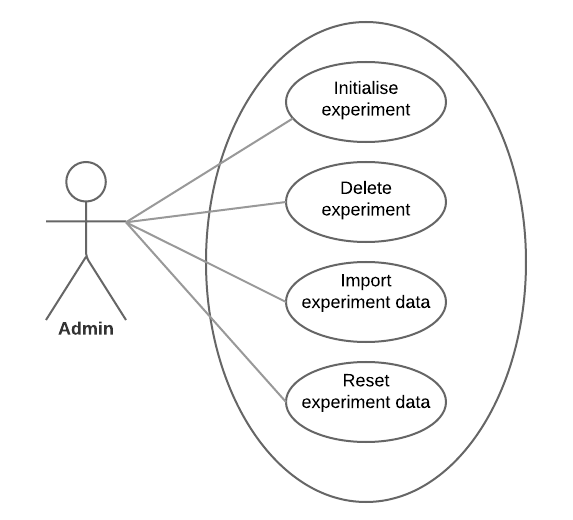
\includegraphics[width=0.5\textwidth]{images/analysis/admin_case}
    \caption{Use cases for admin user}
    \label{fig:admin_case}
\end{figure}

\subsubsection{User}

Figure~\ref{fig:user_case} shows the use cases for the general user role. Users of the system are able to select between the various available experiments and browse the plants and images associated with them. Users are able to add data to plants in the form of tags or key value pair attributes. Users are able to generate graphs from the available data.

\begin{figure}[H]
    \centering
    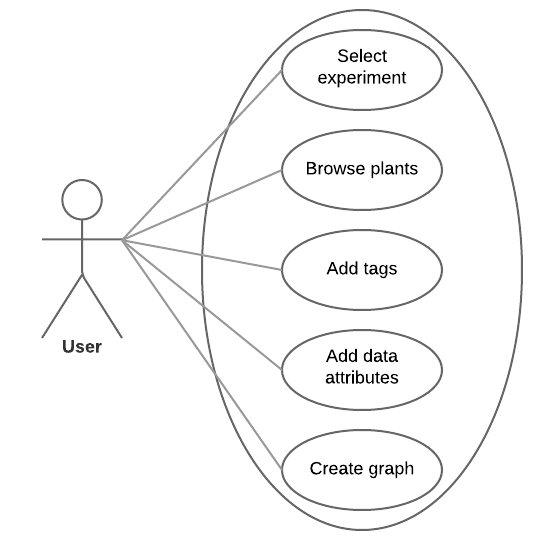
\includegraphics[width=0.5\textwidth]{images/analysis/user_case}
    \caption{Use cases for generic user}
    \label{fig:user_case}
\end{figure}

\section{Process}

Plan driven approaches traditionally associated with software development projects usually expect that all system requirements are understood and collected prior to any further work on design or implementation. A number of factors made such an approach unsuitable for this project, chiefly a lack of domain knowledge made up-front requirement gathering difficult and the requirements themselves were likely to be poorly defined and subject to change. 

The methodology used for the delivery of the project was an agile approach based on the popular SCRUM methodology. For the duration of the project, work would be carried out in time-boxed iterations or `sprints', each a week long. Sprints would begin with a planning session and end with a release of the system software. At the conclusion of each sprint a short retrospective analysis of the sprint would take place, looking at what went well and what could improve for the next iteration. The focus on incremental delivery of working software allowed the project to evolve in an emergent fashion whilst remaining continuously functional as features were prototyped, designed and implemented.  

System requirements were broken down into user stories which in turn were broken down into individual tasks if necessary. As in SCRUM, these stories were held in a backlog until being added into a current or future sprint depending on priority and the goal for a particular sprint. Emergent issues such as priority bugs could easily be incorporated into the wider context of the current sprint if necessary which allowed work to be focused on the most pressing issues. The Jira \cite{jira} issue tracking application was used in support of this process providing an environemnt in which to specify and track user stories,task and sprints, see section~\ref{jira_sec} for further details. 

During a sprint, each day would begin with a quick overview of tasks in the sprint, replicating the `stand-up' meetings common in SCRUM. Work would be commenced or continued on the task deemed highest priority at the time. At the end of each day a short update would often be posted on the project blog available at \url{https://siongriffithsblog.wordpress.com/} summarising the days activity. The blog itself has proven to be a useful part of the process, helping to document certain aspects of the implementation and design that may have otherwise been forgotten.


\subsection{Time Management}
Effective management of time is a key consideration of any reasonable development process model. Partway through the project it was decided to fully adopt the Pomodoro technique \cite{pomodoro}, working in blocks of twenty five minutes with complete focus on the task at hand, referred to as Pomodoros. A five minute break is taken after each successful twenty five minute work block in order to avoid the mental fatigue of attempting to remain focused and productive for an extended amount of time. Taking these regular, short breaks allowed for a higher degree of productivity over the course of a work day.

Having distinct blocks of time in which to complete work compliments the SCRUM approach to effort tracking and estimation. Although not part of the initial process, towards the latter half of the project after gaining a sufficient feel for the possible output of a single Pomodoro, all work was estimated in terms of the Pomodoros required to complete the task. The goal for a given sprint was to achieve sixty Pomodoro and use this figure as the budget for work that could be done. It was fairly difficult to estimate in terms of Pomodoro and often fairly inaccurate, although the productivity aspect certainly works, the more abstract and popular `story-point' method of effort estimation is what would be used if the project was repeated.

Figure ~\ref{fig:pomo1} shows the early Pomodoro tracking during two iterations. A successful Pomodoro would result in a sticker being allocated to that day. It was preferable to have Pomodoro goals for a given sprint rather than concrete work times (for example nine-to-five) since this allowed a great deal of flexibility whilst also maintaining that a weeks worth of work was to be done. Effort could be expended in the beginning of the week in order to have more time later on for example.  

\begin{figure}[H]
    \centering
    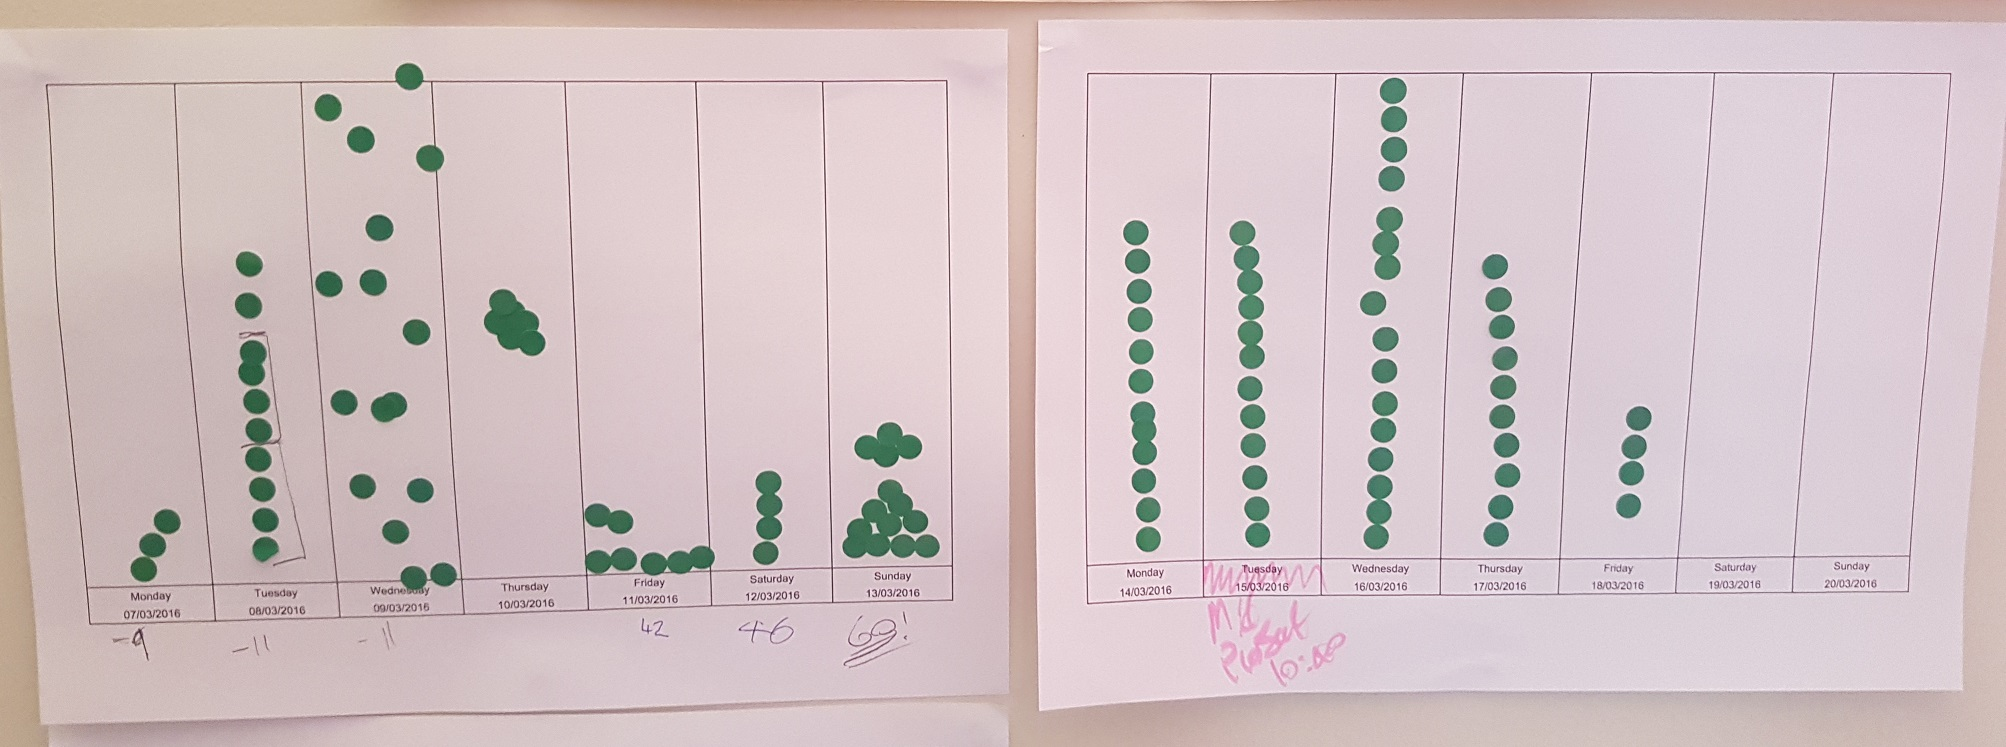
\includegraphics[width=\textwidth]{images/process/pomotrack}
    \caption{Tracking pomodoros}
    \label{fig:pomo1}
\end{figure}


%The process used for the project was an agile based approach similar in style to Scrum although adapted for a project team of one. The process centred around User Stories and short iterations of one week. 

